% Options for packages loaded elsewhere
\PassOptionsToPackage{unicode}{hyperref}
\PassOptionsToPackage{hyphens}{url}
%
\documentclass[
]{article}
\usepackage{lmodern}
\usepackage{amssymb,amsmath}
\usepackage{ifxetex,ifluatex}
\ifnum 0\ifxetex 1\fi\ifluatex 1\fi=0 % if pdftex
  \usepackage[T1]{fontenc}
  \usepackage[utf8]{inputenc}
  \usepackage{textcomp} % provide euro and other symbols
\else % if luatex or xetex
  \usepackage{unicode-math}
  \defaultfontfeatures{Scale=MatchLowercase}
  \defaultfontfeatures[\rmfamily]{Ligatures=TeX,Scale=1}
\fi
% Use upquote if available, for straight quotes in verbatim environments
\IfFileExists{upquote.sty}{\usepackage{upquote}}{}
\IfFileExists{microtype.sty}{% use microtype if available
  \usepackage[]{microtype}
  \UseMicrotypeSet[protrusion]{basicmath} % disable protrusion for tt fonts
}{}
\makeatletter
\@ifundefined{KOMAClassName}{% if non-KOMA class
  \IfFileExists{parskip.sty}{%
    \usepackage{parskip}
  }{% else
    \setlength{\parindent}{0pt}
    \setlength{\parskip}{6pt plus 2pt minus 1pt}}
}{% if KOMA class
  \KOMAoptions{parskip=half}}
\makeatother
\usepackage{xcolor}
\IfFileExists{xurl.sty}{\usepackage{xurl}}{} % add URL line breaks if available
\IfFileExists{bookmark.sty}{\usepackage{bookmark}}{\usepackage{hyperref}}
\hypersetup{
  pdftitle={Frontier 1 : Maps},
  pdfauthor={Claude Grasland},
  hidelinks,
  pdfcreator={LaTeX via pandoc}}
\urlstyle{same} % disable monospaced font for URLs
\usepackage[margin=1in]{geometry}
\usepackage{graphicx}
\makeatletter
\def\maxwidth{\ifdim\Gin@nat@width>\linewidth\linewidth\else\Gin@nat@width\fi}
\def\maxheight{\ifdim\Gin@nat@height>\textheight\textheight\else\Gin@nat@height\fi}
\makeatother
% Scale images if necessary, so that they will not overflow the page
% margins by default, and it is still possible to overwrite the defaults
% using explicit options in \includegraphics[width, height, ...]{}
\setkeys{Gin}{width=\maxwidth,height=\maxheight,keepaspectratio}
% Set default figure placement to htbp
\makeatletter
\def\fps@figure{htbp}
\makeatother
\setlength{\emergencystretch}{3em} % prevent overfull lines
\providecommand{\tightlist}{%
  \setlength{\itemsep}{0pt}\setlength{\parskip}{0pt}}
\setcounter{secnumdepth}{-\maxdimen} % remove section numbering
\usepackage{booktabs}
\usepackage{longtable}
\usepackage{array}
\usepackage{multirow}
\usepackage{wrapfig}
\usepackage{float}
\usepackage{colortbl}
\usepackage{pdflscape}
\usepackage{tabu}
\usepackage{threeparttable}
\usepackage{threeparttablex}
\usepackage[normalem]{ulem}
\usepackage{makecell}
\usepackage{xcolor}

\title{Frontier 1 : Maps}
\author{Claude Grasland}
\date{27/03/2021}

\begin{document}
\maketitle

\hypertarget{data-preparation}{%
\subsection{DATA PREPARATION}\label{data-preparation}}

\hypertarget{load-hypercube}{%
\subsubsection{Load hypercube}\label{load-hypercube}}

We have collected titles of news declared as \emph{international} as
long as we have depicted the existence of at less one foreign country in
the text of the title. In each of the 5 countries, we have selected
three newspapers with national audience and available through mediacloud
database from mid 2013 to mid 2020.

\begin{verbatim}
##              who      N
## 1: fr_FRA_lmonde 104176
## 2: fr_FRA_figaro 240318
## 3: fr_FRA_lacroi 249445
\end{verbatim}

\begin{verbatim}
##              who      N
## 1: de_DEU_suddeu  83774
## 2: de_DEU_diewel 112065
## 3: de_DEU_frankf 103111
\end{verbatim}

\begin{verbatim}
##              who      N
## 1: en_GBR_dailyt  62657
## 2: en_GBR_indept 156128
## 3: en_GBR_guardi 171949
\end{verbatim}

\begin{verbatim}
##              who      N
## 1: it_ITA_stampa  90059
## 2: it_ITA_messag 104909
## 3: it_ITA_repubb  86468
\end{verbatim}

\begin{verbatim}
##              who      N
## 1: es_ESP_abcxxx 280895
## 2:  es_ESP_mundo  38457
## 3: es_ESP_percat 142259
\end{verbatim}

\hypertarget{compute-news-flow-between-host-and-guest-countries-and-modelize}{%
\subsubsection{Compute news flow between host and guest countries and
modelize}\label{compute-news-flow-between-host-and-guest-countries-and-modelize}}

What is the distribution of foreign news in each country ? We aggregate
news for the whole period by host and guest countries. Then we modelize
the expected number of news Fij through a double contrtaint model based
on the marginal sums of news produced by each host country (i) about
each guest country (j). Estimation are realized by a \textbf{poisson
regression model}.

\hypertarget{prepare-world-map}{%
\subsection{Prepare world map}\label{prepare-world-map}}

We use the world map elaborated by Romain Leconte for his PhD and we
choose the full version for centroid and the simplified version for
drawing maps. We use a Lambrt Azimuthal Projection centerd on Paris with
the formulata \emph{crs = ``+proj=laea +x\_0=0 +y\_0=0 +lon\_0=2
+lat\_0=49''}.

We try(as an experiment) to use the new package \texttt{mapsf}
elaborated by RIATE which is the follower of the well known package
\texttt{cartography}.

\url{https://riatelab.github.io/mapsf/articles/mapsf.html}

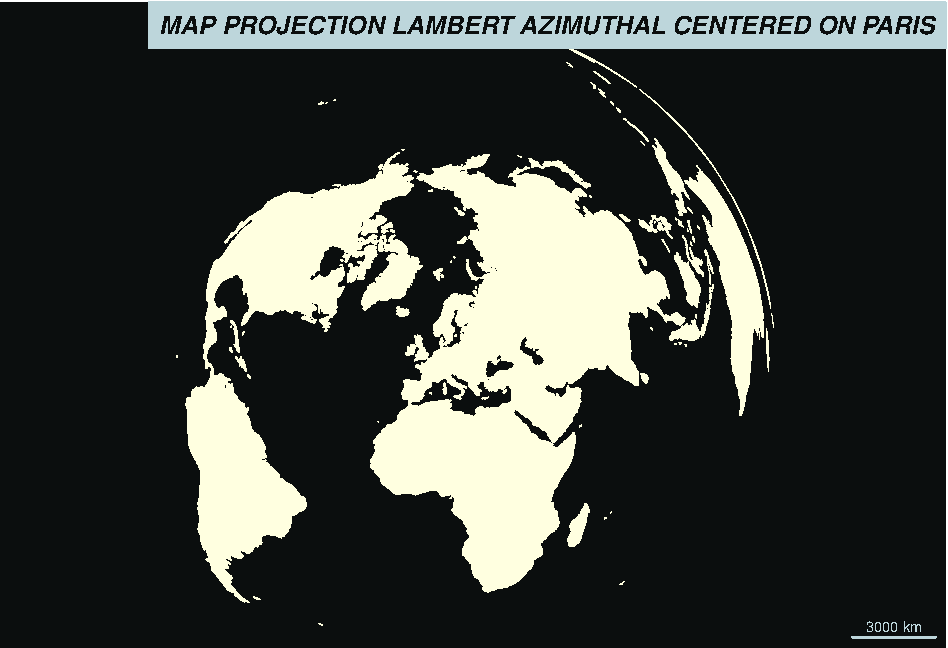
\includegraphics{Part2_maps_files/figure-latex/unnamed-chunk-4-1.pdf}

\begin{center}\rule{0.5\linewidth}{0.5pt}\end{center}

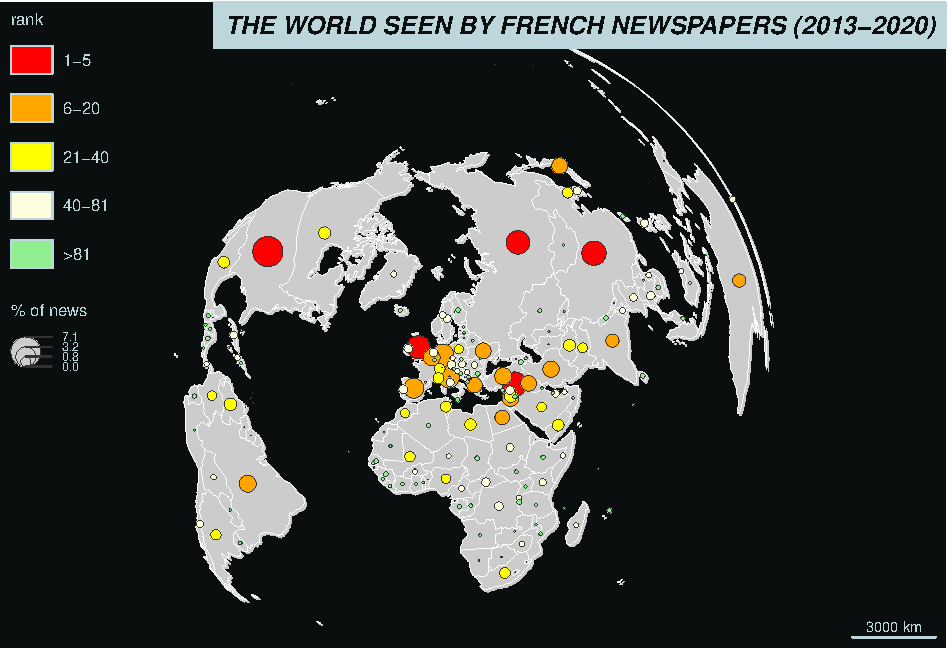
\includegraphics{Part2_maps_files/figure-latex/unnamed-chunk-5-1.pdf}

\begin{table}

\caption{\label{tab:unnamed-chunk-6}Top countries mentionned by french newspapers (2013-2020)}
\centering
\begin{tabular}[t]{r|l|l|r|r|r}
\hline
Rank & Code & Country & Nb.of news & \% & Cum. \%\\
\hline
1 & USA & United States of America & 13583 & 7.1 & 7.1\\
\hline
2 & SYR & Syria & 9025 & 4.7 & 11.7\\
\hline
3 & CHN & China & 8900 & 4.6 & 16.4\\
\hline
4 & RUS & Russia & 8324 & 4.3 & 20.7\\
\hline
5 & GBR & United Kingdom & 7888 & 4.1 & 24.8\\
\hline
6 & DEU & Germany & 7740 & 4.0 & 28.8\\
\hline
7 & ITA & Italy & 6414 & 3.3 & 32.1\\
\hline
8 & ESP & Spain & 6100 & 3.2 & 35.3\\
\hline
9 & TUR & Turkey & 4460 & 2.3 & 37.6\\
\hline
10 & BRA & Brazil & 4376 & 2.3 & 39.9\\
\hline
11 & BEL & Belgium & 4249 & 2.2 & 42.1\\
\hline
12 & ISR & Israel & 4202 & 2.2 & 44.3\\
\hline
13 & IRN & Iran & 4083 & 2.1 & 46.4\\
\hline
14 & JPN & Japan & 3941 & 2.0 & 48.4\\
\hline
15 & UKR & Ukraine & 3832 & 2.0 & 50.4\\
\hline
\end{tabular}
\end{table}

\begin{center}\rule{0.5\linewidth}{0.5pt}\end{center}

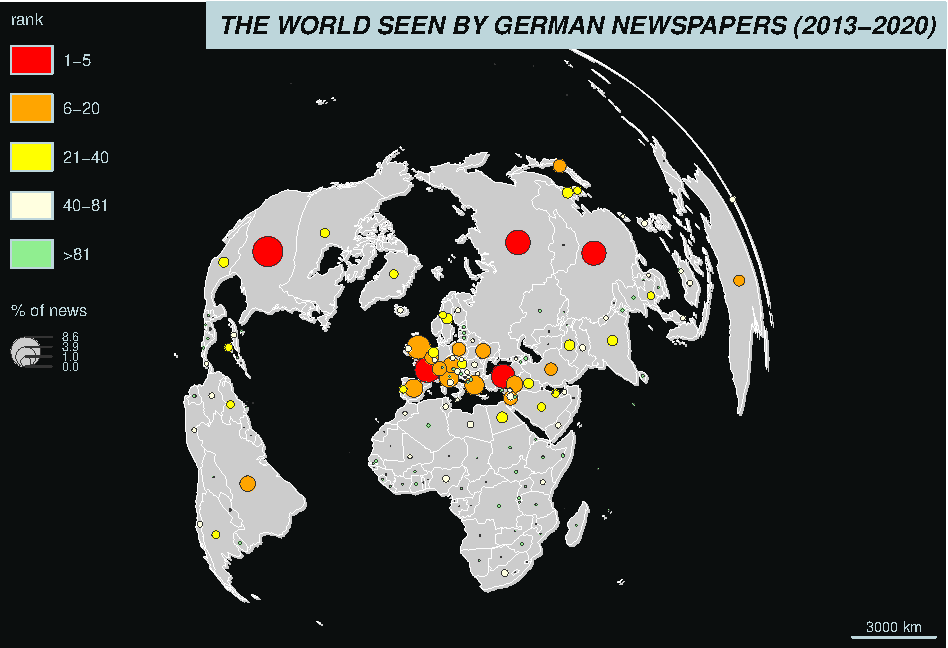
\includegraphics{Part2_maps_files/figure-latex/unnamed-chunk-7-1.pdf}

\begin{table}

\caption{\label{tab:unnamed-chunk-8}Top countries mentionned by german newspapers (2013-2020)}
\centering
\begin{tabular}[t]{r|l|l|r|r|r}
\hline
Rank & Code & Country & Nb.of news & \% & Cum. \%\\
\hline
1 & USA & United States of America & 8796 & 8.6 & 8.6\\
\hline
2 & FRA & France & 6241 & 6.1 & 14.7\\
\hline
3 & RUS & Russia & 5876 & 5.8 & 20.5\\
\hline
4 & CHN & China & 5677 & 5.6 & 26.0\\
\hline
5 & TUR & Turkey & 5483 & 5.4 & 31.4\\
\hline
6 & GBR & United Kingdom & 5413 & 5.3 & 36.7\\
\hline
7 & ITA & Italy & 3749 & 3.7 & 40.4\\
\hline
8 & GRC & Greece & 3659 & 3.6 & 43.9\\
\hline
9 & ESP & Spain & 3288 & 3.2 & 47.2\\
\hline
10 & SYR & Syria & 2719 & 2.7 & 49.8\\
\hline
11 & AUT & Austria & 2529 & 2.5 & 52.3\\
\hline
12 & BRA & Brazil & 2366 & 2.3 & 54.6\\
\hline
13 & UKR & Ukraine & 2180 & 2.1 & 56.8\\
\hline
14 & CHE & Switzerland & 2029 & 2.0 & 58.7\\
\hline
15 & ISR & Israel & 1925 & 1.9 & 60.6\\
\hline
\end{tabular}
\end{table}

\begin{center}\rule{0.5\linewidth}{0.5pt}\end{center}

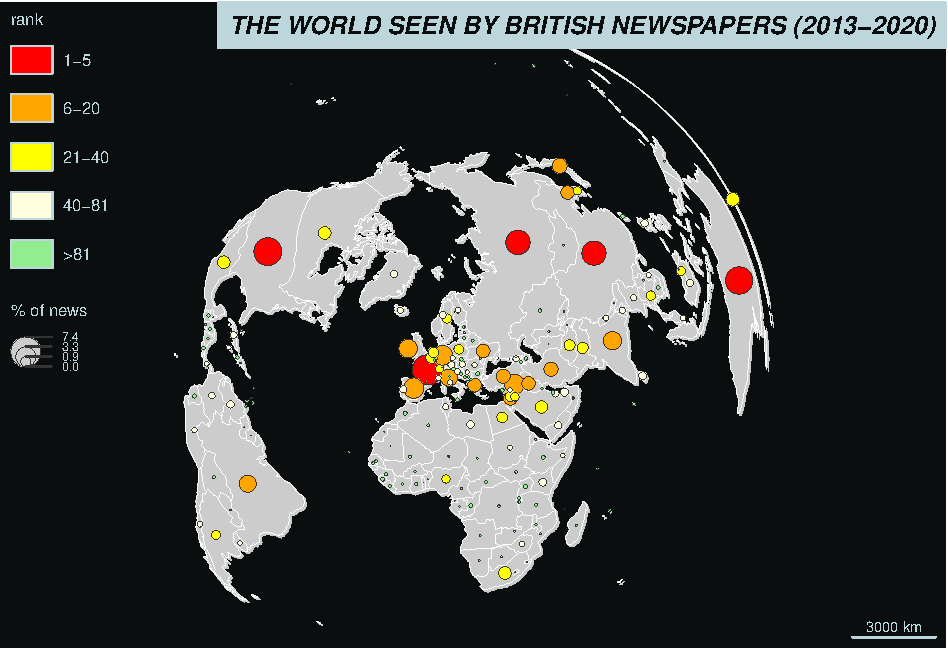
\includegraphics{Part2_maps_files/figure-latex/unnamed-chunk-9-1.pdf}

\begin{table}

\caption{\label{tab:unnamed-chunk-10}Top countries mentionned by british newspapers (2013-2020)}
\centering
\begin{tabular}[t]{r|l|l|r|r|r}
\hline
Rank & Code & Country & Nb.of news & \% & Cum. \%\\
\hline
1 & FRA & France & 17788 & 7.4 & 7.4\\
\hline
2 & USA & United States of America & 15235 & 6.3 & 13.7\\
\hline
3 & AUS & Australia & 14631 & 6.1 & 19.8\\
\hline
4 & RUS & Russia & 11646 & 4.8 & 24.6\\
\hline
5 & CHN & China & 11449 & 4.8 & 29.4\\
\hline
6 & ESP & Spain & 8229 & 3.4 & 32.8\\
\hline
7 & SYR & Syria & 7882 & 3.3 & 36.1\\
\hline
8 & DEU & Germany & 7770 & 3.2 & 39.3\\
\hline
9 & IRL & Ireland & 6837 & 2.8 & 42.1\\
\hline
10 & IND & India & 6652 & 2.8 & 44.9\\
\hline
11 & ITA & Italy & 5850 & 2.4 & 47.3\\
\hline
12 & BRA & Brazil & 5806 & 2.4 & 49.7\\
\hline
13 & JPN & Japan & 4430 & 1.8 & 51.6\\
\hline
14 & IRN & Iran & 3998 & 1.7 & 53.2\\
\hline
15 & TUR & Turkey & 3955 & 1.6 & 54.9\\
\hline
\end{tabular}
\end{table}

\begin{center}\rule{0.5\linewidth}{0.5pt}\end{center}

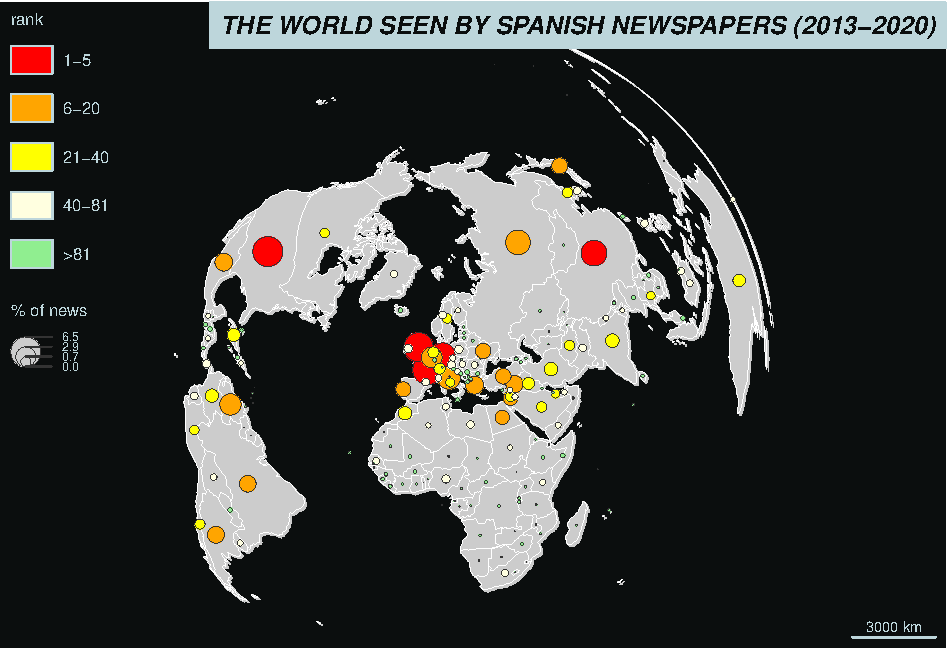
\includegraphics{Part2_maps_files/figure-latex/unnamed-chunk-11-1.pdf}

\begin{table}

\caption{\label{tab:unnamed-chunk-12}Top countries mentionned by spanish newspapers (2013-2020)}
\centering
\begin{tabular}[t]{r|l|l|r|r|r}
\hline
Rank & Code & Country & Nb.of news & \% & Cum. \%\\
\hline
1 & USA & United States of America & 9045 & 6.5 & 6.5\\
\hline
2 & FRA & France & 8842 & 6.3 & 12.8\\
\hline
3 & GBR & United Kingdom & 8548 & 6.1 & 18.9\\
\hline
4 & CHN & China & 6603 & 4.7 & 23.6\\
\hline
5 & DEU & Germany & 6195 & 4.4 & 28.0\\
\hline
6 & RUS & Russia & 6125 & 4.4 & 32.4\\
\hline
7 & ITA & Italy & 5372 & 3.8 & 36.2\\
\hline
8 & VEN & Venezuela & 4630 & 3.3 & 39.5\\
\hline
9 & BEL & Belgium & 4396 & 3.1 & 42.6\\
\hline
10 & GRC & Greece & 3276 & 2.3 & 45.0\\
\hline
11 & MEX & Mexico & 3148 & 2.2 & 47.2\\
\hline
12 & SYR & Syria & 3043 & 2.2 & 49.4\\
\hline
13 & ARG & Argentina & 2918 & 2.1 & 51.5\\
\hline
14 & BRA & Brazil & 2773 & 2.0 & 53.5\\
\hline
15 & JPN & Japan & 2612 & 1.9 & 55.3\\
\hline
\end{tabular}
\end{table}

\begin{center}\rule{0.5\linewidth}{0.5pt}\end{center}

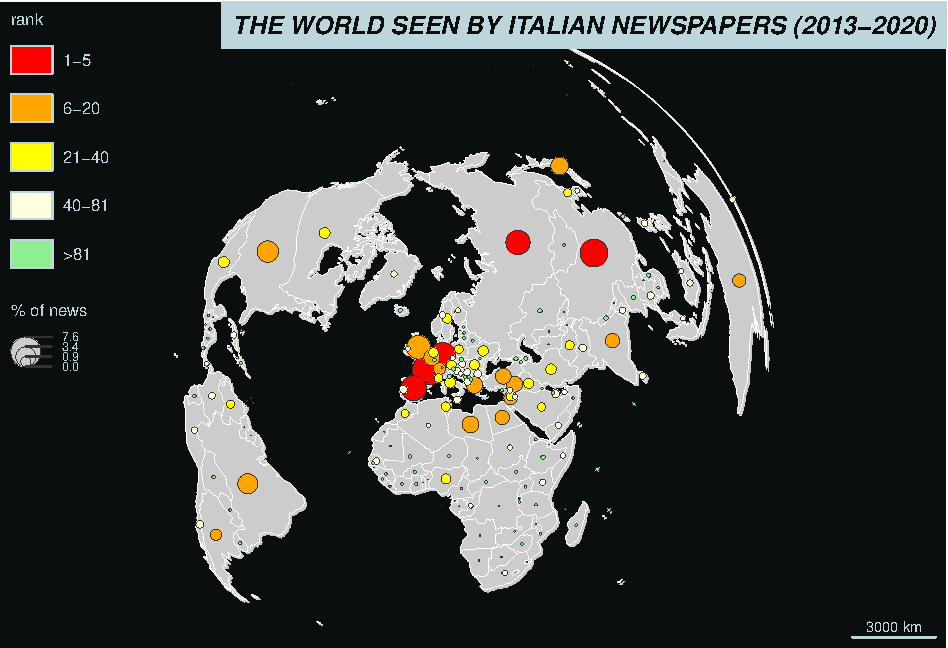
\includegraphics{Part2_maps_files/figure-latex/unnamed-chunk-13-1.pdf}

\begin{table}

\caption{\label{tab:unnamed-chunk-14}Top countries mentionned by italian newspapers (2013-2020)}
\centering
\begin{tabular}[t]{r|l|l|r|r|r}
\hline
Rank & Code & Country & Nb.of news & \% & Cum. \%\\
\hline
1 & FRA & France & 6164 & 7.6 & 7.6\\
\hline
2 & CHN & China & 5256 & 6.5 & 14.1\\
\hline
3 & DEU & Germany & 4437 & 5.5 & 19.6\\
\hline
4 & ESP & Spain & 4311 & 5.3 & 24.9\\
\hline
5 & RUS & Russia & 3975 & 4.9 & 29.8\\
\hline
6 & GBR & United Kingdom & 3853 & 4.8 & 34.5\\
\hline
7 & USA & United States of America & 3183 & 3.9 & 38.5\\
\hline
8 & BRA & Brazil & 2788 & 3.4 & 41.9\\
\hline
9 & JPN & Japan & 2148 & 2.6 & 44.5\\
\hline
10 & LBY & Libya & 1923 & 2.4 & 46.9\\
\hline
11 & GRC & Greece & 1862 & 2.3 & 49.2\\
\hline
12 & BEL & Belgium & 1774 & 2.2 & 51.4\\
\hline
13 & SYR & Syria & 1738 & 2.1 & 53.5\\
\hline
14 & TUR & Turkey & 1719 & 2.1 & 55.7\\
\hline
15 & IND & India & 1431 & 1.8 & 57.4\\
\hline
\end{tabular}
\end{table}

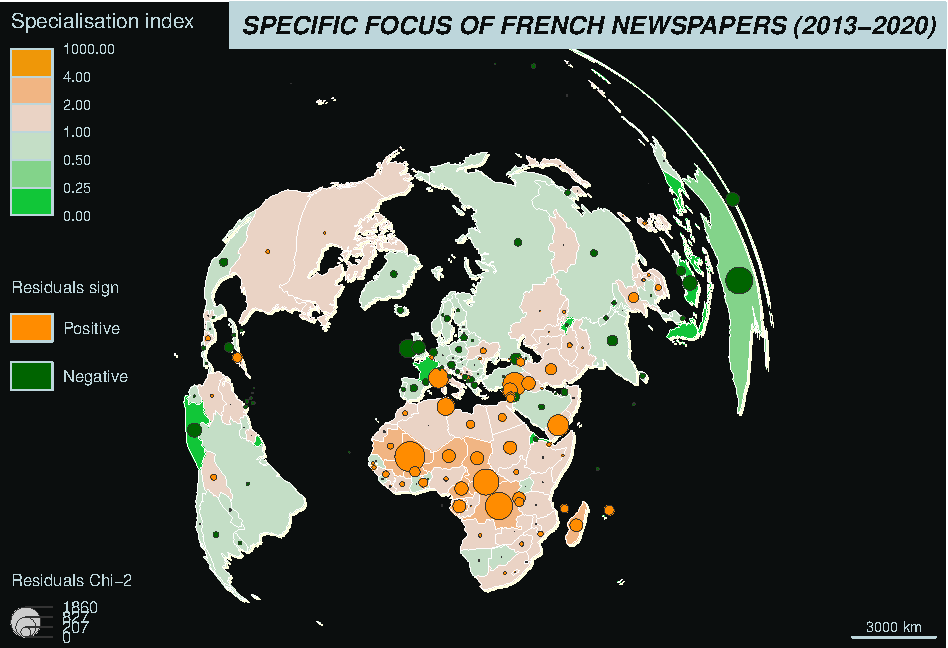
\includegraphics{Part2_maps_files/figure-latex/unnamed-chunk-15-1.pdf}

\begin{table}

\caption{\label{tab:unnamed-chunk-16}Most significant positive residuals of French Newspapers}
\centering
\begin{tabular}[t]{l|l|l|r|r|r|r|r}
\hline
  & Code & Country & Observed & Estimated & Difference & Ratio & Chi-square\\
\hline
1 & MLI & Mali & 1641 & 592 & 1049 & 2.77 & 1860.3\\
\hline
2 & COD & Dem. Rep. Congo & 1122 & 369 & 753 & 3.04 & 1534.1\\
\hline
3 & CAF & Central African Rep. & 1105 & 379 & 726 & 2.91 & 1387.4\\
\hline
4 & SYR & Syria & 9025 & 6343 & 2682 & 1.42 & 1133.8\\
\hline
5 & YEM & Yemen & 2005 & 1033 & 972 & 1.94 & 915.8\\
\hline
6 & MCO & Monaco & 1728 & 877 & 851 & 1.97 & 826.9\\
\hline
7 & TUN & Tunisia & 1842 & 1030 & 812 & 1.79 & 640.8\\
\hline
8 & LBN & Lebanon & 1113 & 599 & 514 & 1.86 & 440.9\\
\hline
9 & IRQ & Iraq & 3756 & 2737 & 1019 & 1.37 & 379.0\\
\hline
10 & CMR & Cameroon & 531 & 234 & 297 & 2.27 & 377.4\\
\hline
11 & TCD & Chad & 326 & 119 & 207 & 2.75 & 363.3\\
\hline
12 & SDN & Sudan & 947 & 518 & 429 & 1.83 & 355.4\\
\hline
13 & NER & Niger & 385 & 153 & 232 & 2.51 & 350.0\\
\hline
14 & GAB & Gabon & 269 & 92 & 177 & 2.92 & 340.5\\
\hline
15 & MDG & Madagascar & 394 & 161 & 233 & 2.45 & 339.1\\
\hline
\end{tabular}
\end{table}

\begin{center}\rule{0.5\linewidth}{0.5pt}\end{center}

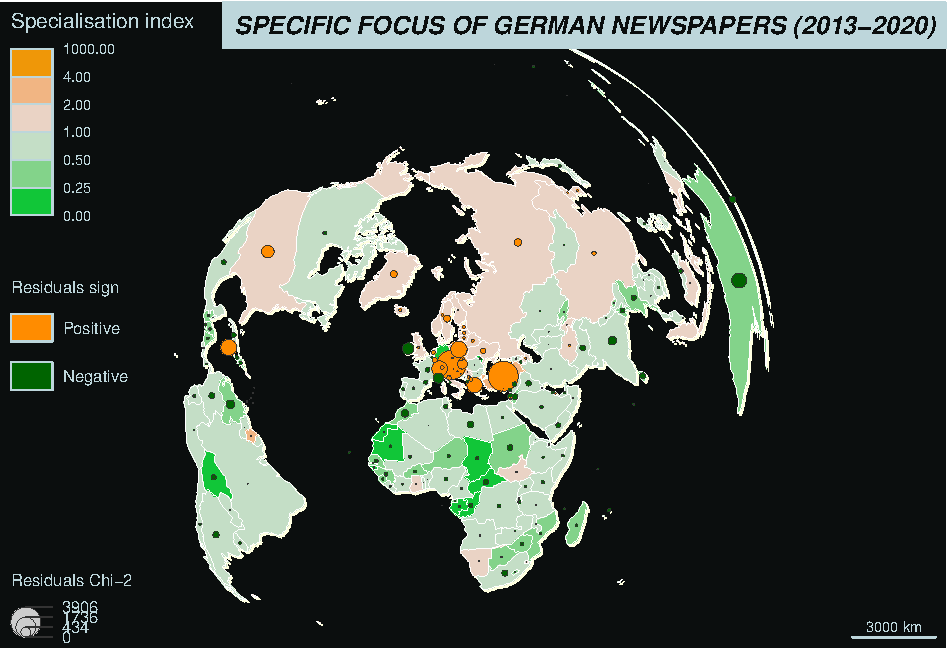
\includegraphics{Part2_maps_files/figure-latex/unnamed-chunk-17-1.pdf}

\begin{table}

\caption{\label{tab:unnamed-chunk-18}Most significant positive residuals of German Newspapers}
\centering
\begin{tabular}[t]{l|l|l|r|r|r|r|r}
\hline
  & Code & Country & Observed & Estimated & Difference & Ratio & Chi-square\\
\hline
1 & TUR & Turkey & 5483 & 2413 & 3070 & 2.27 & 3905.8\\
\hline
2 & AUT & Austria & 2529 & 803 & 1726 & 3.15 & 3706.7\\
\hline
3 & POL & Poland & 1828 & 838 & 990 & 2.18 & 1168.0\\
\hline
4 & JAM & Jamaica & 586 & 161 & 425 & 3.65 & 1127.9\\
\hline
5 & CHE & Switzerland & 2029 & 1000 & 1029 & 2.03 & 1058.9\\
\hline
6 & GRC & Greece & 3659 & 2165 & 1494 & 1.69 & 1031.1\\
\hline
7 & USA & United States of America & 8796 & 6667 & 2129 & 1.32 & 680.0\\
\hline
8 & HUN & Hungary & 848 & 422 & 426 & 2.01 & 430.8\\
\hline
9 & RUS & Russia & 5876 & 4808 & 1068 & 1.22 & 237.2\\
\hline
10 & SWE & Sweden & 1126 & 732 & 394 & 1.54 & 212.0\\
\hline
11 & DNK & Denmark & 731 & 430 & 301 & 1.70 & 211.4\\
\hline
12 & UKR & Ukraine & 2180 & 1716 & 464 & 1.27 & 125.7\\
\hline
13 & LUX & Luxembourg & 231 & 115 & 116 & 2.00 & 116.1\\
\hline
14 & ITA & Italy & 3749 & 3197 & 552 & 1.17 & 95.3\\
\hline
15 & CHN & China & 5677 & 5067 & 610 & 1.12 & 73.3\\
\hline
\end{tabular}
\end{table}

\begin{center}\rule{0.5\linewidth}{0.5pt}\end{center}

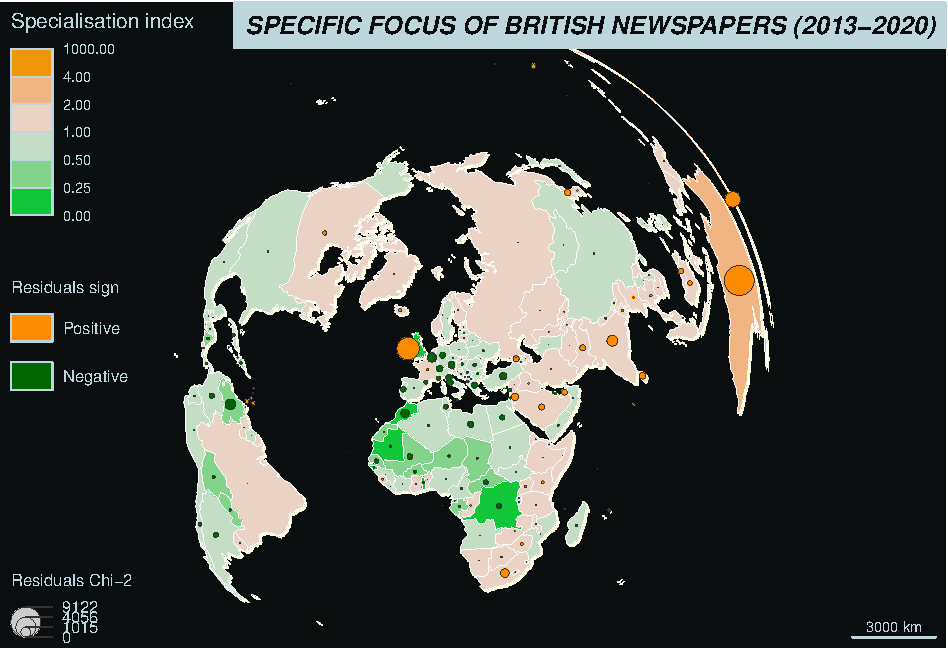
\includegraphics{Part2_maps_files/figure-latex/unnamed-chunk-19-1.pdf}

\begin{table}

\caption{\label{tab:unnamed-chunk-20}Most significant positive residuals of British Newspapers}
\centering
\begin{tabular}[t]{l|l|l|r|r|r|r|r}
\hline
  & Code & Country & Observed & Estimated & Difference & Ratio & Chi-square\\
\hline
1 & AUS & Australia & 14631 & 6772 & 7859 & 2.16 & 9122.1\\
\hline
2 & IRL & Ireland & 6837 & 2949 & 3888 & 2.32 & 5124.2\\
\hline
3 & NZL & New Zealand & 3569 & 1603 & 1966 & 2.23 & 2413.0\\
\hline
4 & IND & India & 6652 & 4367 & 2285 & 1.52 & 1196.1\\
\hline
5 & ZAF & South Africa & 3163 & 1953 & 1210 & 1.62 & 749.5\\
\hline
6 & JOR & Jordan & 1400 & 749 & 651 & 1.87 & 566.1\\
\hline
7 & LKA & Sri Lanka & 1232 & 681 & 551 & 1.81 & 444.9\\
\hline
8 & PRK & North Korea & 3608 & 2595 & 1013 & 1.39 & 395.1\\
\hline
9 & GEO & Georgia & 770 & 387 & 383 & 1.99 & 378.5\\
\hline
10 & PAK & Pakistan & 2493 & 1702 & 791 & 1.46 & 367.7\\
\hline
11 & SAU & Saudi Arabia & 3027 & 2142 & 885 & 1.41 & 365.4\\
\hline
12 & ARE & United Arab Emirates & 1313 & 791 & 522 & 1.66 & 344.6\\
\hline
13 & MYS & Malaysia & 1493 & 942 & 551 & 1.59 & 322.5\\
\hline
14 & NRU & Nauru & 188 & 65 & 123 & 2.89 & 233.1\\
\hline
15 & IDN & Indonesia & 1173 & 758 & 415 & 1.55 & 226.6\\
\hline
\end{tabular}
\end{table}

\begin{center}\rule{0.5\linewidth}{0.5pt}\end{center}

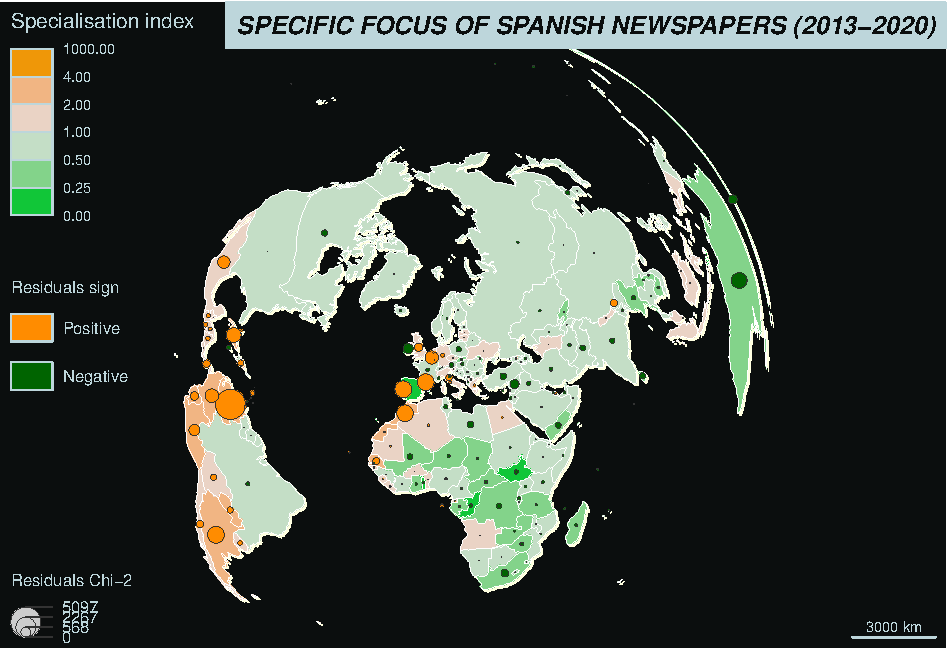
\includegraphics{Part2_maps_files/figure-latex/unnamed-chunk-21-1.pdf}

\begin{table}

\caption{\label{tab:unnamed-chunk-22}Most significant positive residuals of Spanish Newspapers}
\centering
\begin{tabular}[t]{l|l|l|r|r|r|r|r}
\hline
  & Code & Country & Observed & Estimated & Difference & Ratio & Chi-square\\
\hline
1 & VEN & Venezuela & 4630 & 1693 & 2937 & 2.74 & 5097.0\\
\hline
2 & ARG & Argentina & 2918 & 1411 & 1507 & 2.07 & 1611.1\\
\hline
3 & AND & Andorra & 562 & 121 & 441 & 4.63 & 1601.7\\
\hline
4 & PRT & Portugal & 2273 & 1007 & 1266 & 2.26 & 1591.3\\
\hline
5 & MAR & Morocco & 1808 & 735 & 1073 & 2.46 & 1564.0\\
\hline
6 & CUB & Cuba & 1759 & 778 & 981 & 2.26 & 1235.3\\
\hline
7 & COL & Colombia & 1811 & 861 & 950 & 2.10 & 1047.7\\
\hline
8 & BEL & Belgium & 4396 & 2749 & 1647 & 1.60 & 987.5\\
\hline
9 & MEX & Mexico & 3148 & 1868 & 1280 & 1.69 & 877.7\\
\hline
10 & PER & Peru & 889 & 377 & 512 & 2.36 & 693.8\\
\hline
11 & ECU & Ecuador & 583 & 257 & 326 & 2.27 & 412.9\\
\hline
12 & GBR & United Kingdom & 8548 & 6887 & 1661 & 1.24 & 400.6\\
\hline
13 & PAN & Panama & 704 & 362 & 342 & 1.94 & 322.6\\
\hline
14 & CHL & Chile & 1031 & 601 & 430 & 1.71 & 306.8\\
\hline
15 & SEN & Senegal & 535 & 260 & 275 & 2.06 & 291.8\\
\hline
\end{tabular}
\end{table}

\begin{center}\rule{0.5\linewidth}{0.5pt}\end{center}

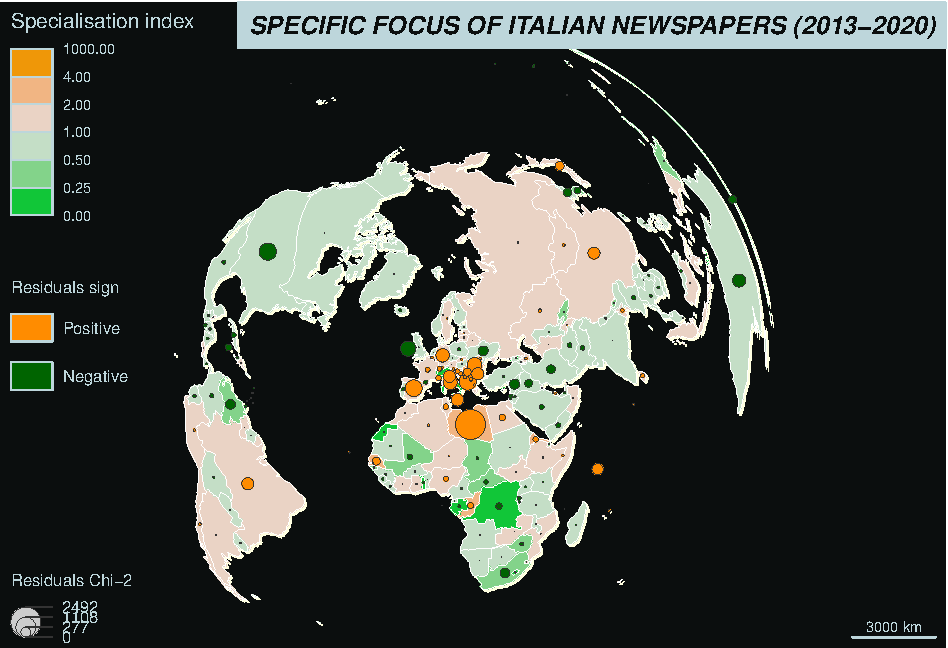
\includegraphics{Part2_maps_files/figure-latex/unnamed-chunk-23-1.pdf}

\begin{table}

\caption{\label{tab:unnamed-chunk-24}Most significant positive residuals of Italian Newspapers}
\centering
\begin{tabular}[t]{l|l|l|r|r|r|r|r}
\hline
  & Code & Country & Observed & Estimated & Difference & Ratio & Chi-square\\
\hline
1 & LBY & Libya & 1923 & 650 & 1273 & 2.96 & 2492.1\\
\hline
2 & ALB & Albania & 393 & 102 & 291 & 3.84 & 825.3\\
\hline
3 & ESP & Spain & 4311 & 2825 & 1486 & 1.53 & 781.7\\
\hline
4 & ROU & Romania & 698 & 285 & 413 & 2.45 & 596.1\\
\hline
5 & VAT & Vatican & 833 & 379 & 454 & 2.20 & 543.1\\
\hline
6 & DEU & Germany & 4437 & 3178 & 1259 & 1.40 & 498.9\\
\hline
7 & MLT & Malta & 388 & 141 & 247 & 2.75 & 431.3\\
\hline
8 & SMR & San Marino & 135 & 28 & 107 & 4.89 & 418.2\\
\hline
9 & BGR & Bulgaria & 412 & 157 & 255 & 2.63 & 416.0\\
\hline
10 & BRA & Brazil & 2788 & 1907 & 881 & 1.46 & 407.1\\
\hline
11 & CHN & China & 5256 & 3989 & 1267 & 1.32 & 402.2\\
\hline
12 & SYC & Seychelles & 100 & 19 & 81 & 5.34 & 352.3\\
\hline
13 & JPN & Japan & 2148 & 1563 & 585 & 1.37 & 219.3\\
\hline
14 & SEN & Senegal & 316 & 150 & 166 & 2.11 & 184.6\\
\hline
15 & SRB & Serbia & 347 & 173 & 174 & 2.01 & 175.0\\
\hline
\end{tabular}
\end{table}

\begin{center}\rule{0.5\linewidth}{0.5pt}\end{center}

\end{document}
